\section{ Messung von Amplituden- und Phasengang der Filterschaltungen }









\subsection{Amplitudengänge (mit Phasengängen) von Butterworth-, Tschebyscheff- und Bessel-Tiefpass gemeinsam in einem Plot über logarithmischer Frequenzachse, Frequenzbereich 100Hz...20kHz („AktFilt Ampl & Phase.set“).}




\subsection{Phasengänge von Butterworth-, Tschebyscheff- und Bessel-Tiefpass gemeinsam in einem Plot über linearer Frequenzachse, Frequenzbereich 100Hz...4kHz. }


% grafik einbinden
\begin{figure}[H]
    \begin{center}
        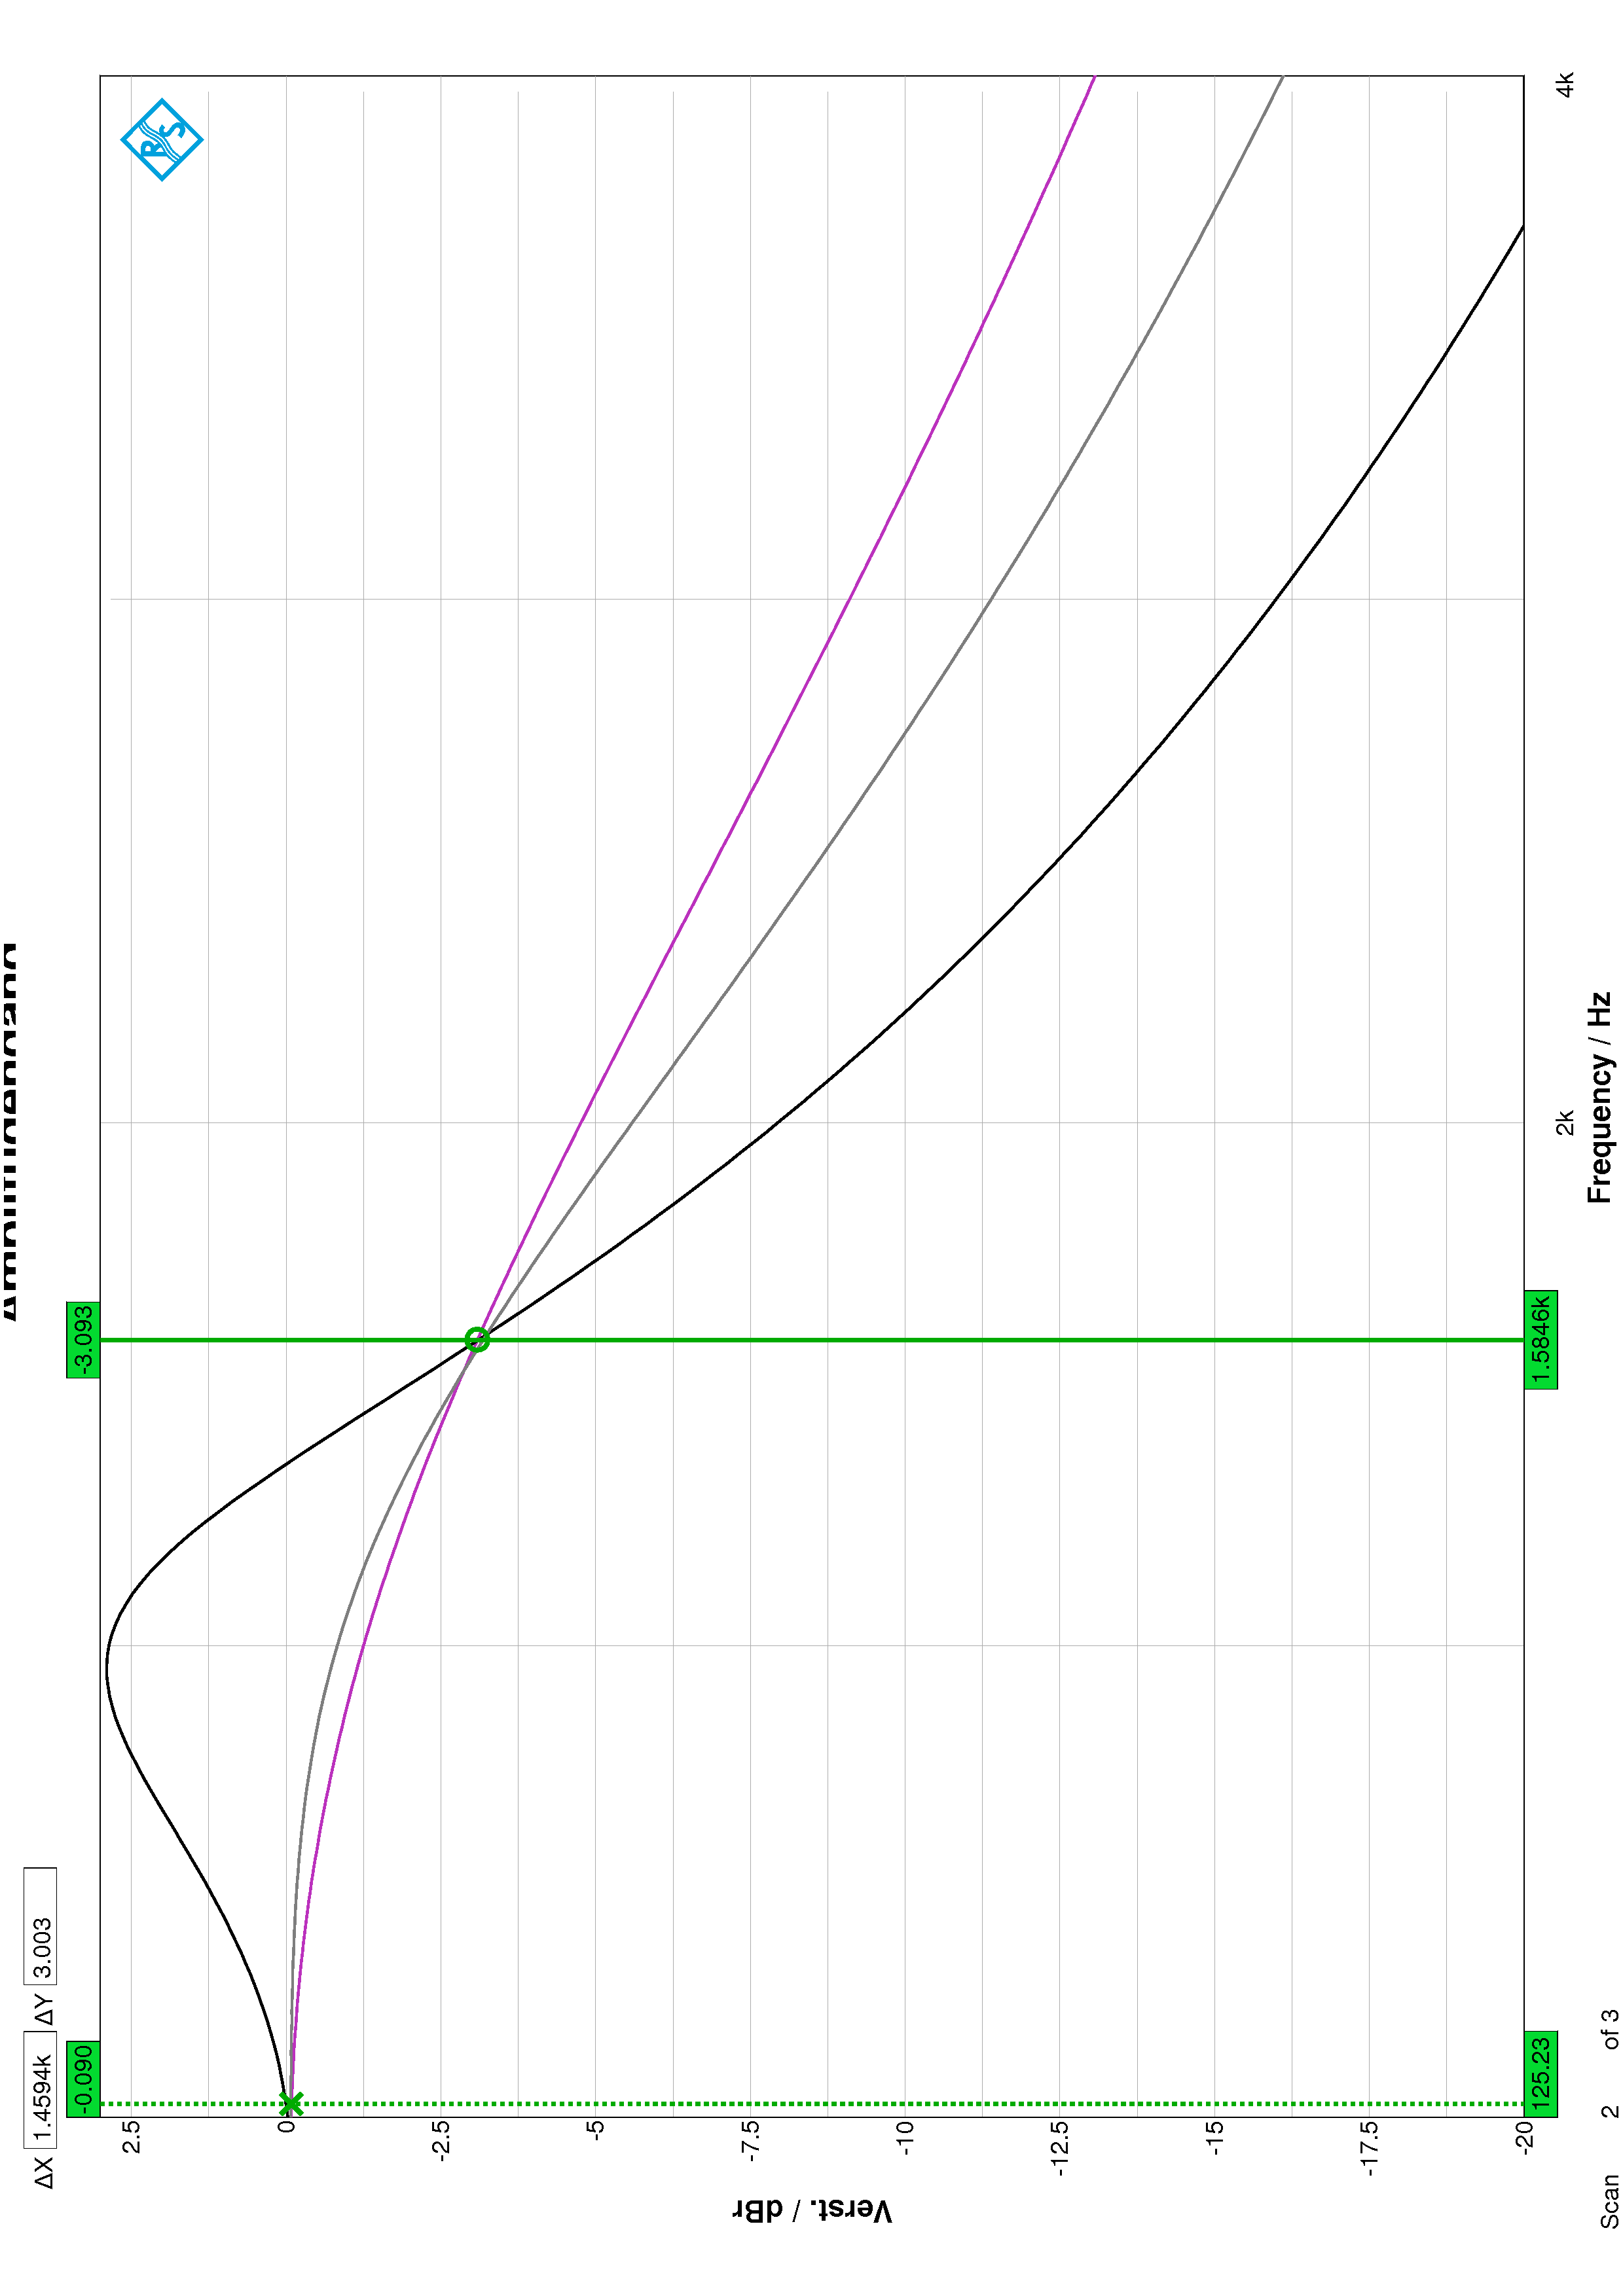
\includegraphics[width=0.8\textwidth, angle =-90]{img/3.2 Amplitudengang linear.png}
        \caption{Amplitudengang linear}
        \label{fig:A1_label}
    \end{center}
\end{figure}
+

% grafik einbinden
\begin{figure}[H]
    \begin{center}
        \includegraphics[width=0.8\textwidth, angle =-90]{img/3.2 Phasengänge linear.png}
        \caption{Phasengänge linear}
        \label{fig:A1_label}
    \end{center}
\end{figure}




\subsection{Amplitudengänge (mit Phasengängen) von Butterworth-, Tschebyscheff- und BesselHochpass gemeinsam in einem Plot über logarithmischer Frequenzachse, Frequenzbereich 100Hz...20kHz. }

% grafik einbinden
\begin{figure}[H]
    \begin{center}
        \includegraphics[width=0.8\textwidth, angle =-90]{img/3.3 Amplitudengänge HP log.png}
        \caption{\imgfilename}
        \label{fig:A1_label}
    \end{center}
\end{figure}
% grafik einbinden
\begin{figure}[H]
    \begin{center}
        \includegraphics[width=0.8\textwidth, angle =-90]{img/3.3 Phasengänge HP log.png}
        \caption{\imgfilename}
        \label{fig:A1_label}
    \end{center}
\end{figure}





\subsection{Amplitudengänge (mit Phasengängen) von Bandpass und Bandsperre gemeinsam in einem Plot über logarithmischer Frequenzachse, Frequenzbereich 1kHz...2,5kHz. }
 

%multi figure
\begin{figure}[h]
\begin{center}
\subfloat[Amplitudengang Bandpass]{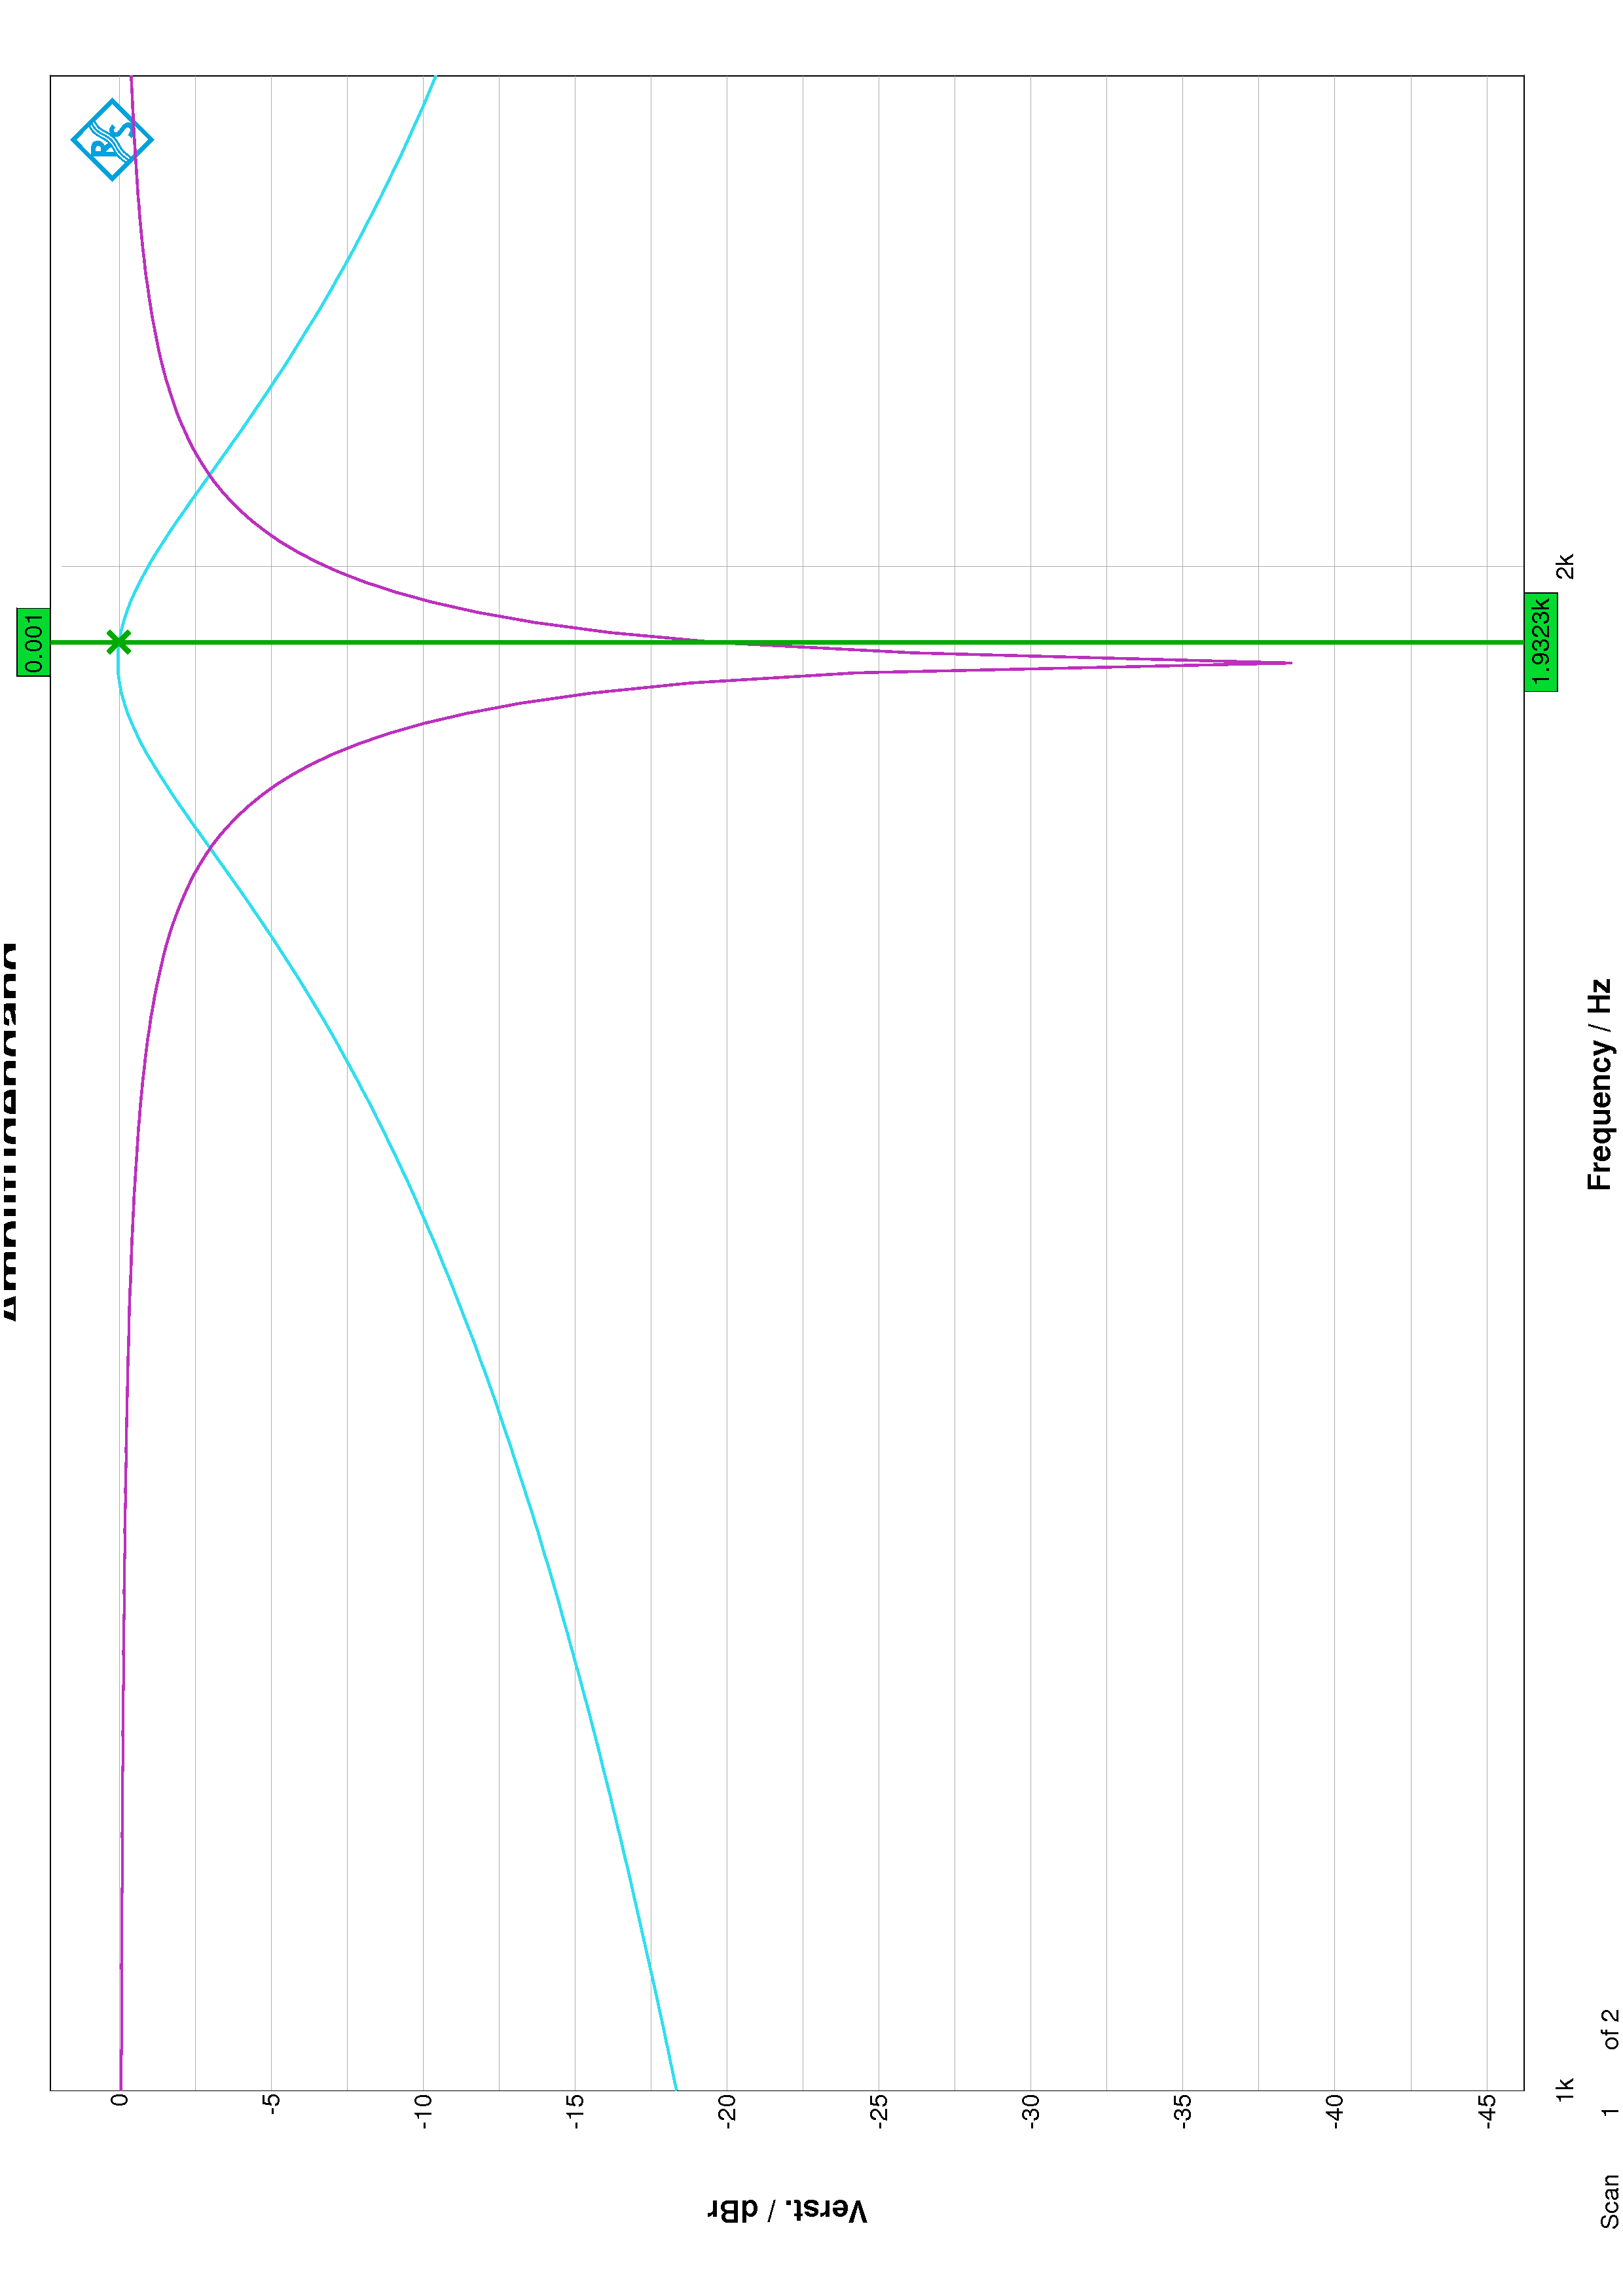
\includegraphics[width = \textwidth/3, angle =-90]{img/3.4 Amplitudengang Bandpass.png}}  
\subfloat[Amplitudengang Bandsperre]{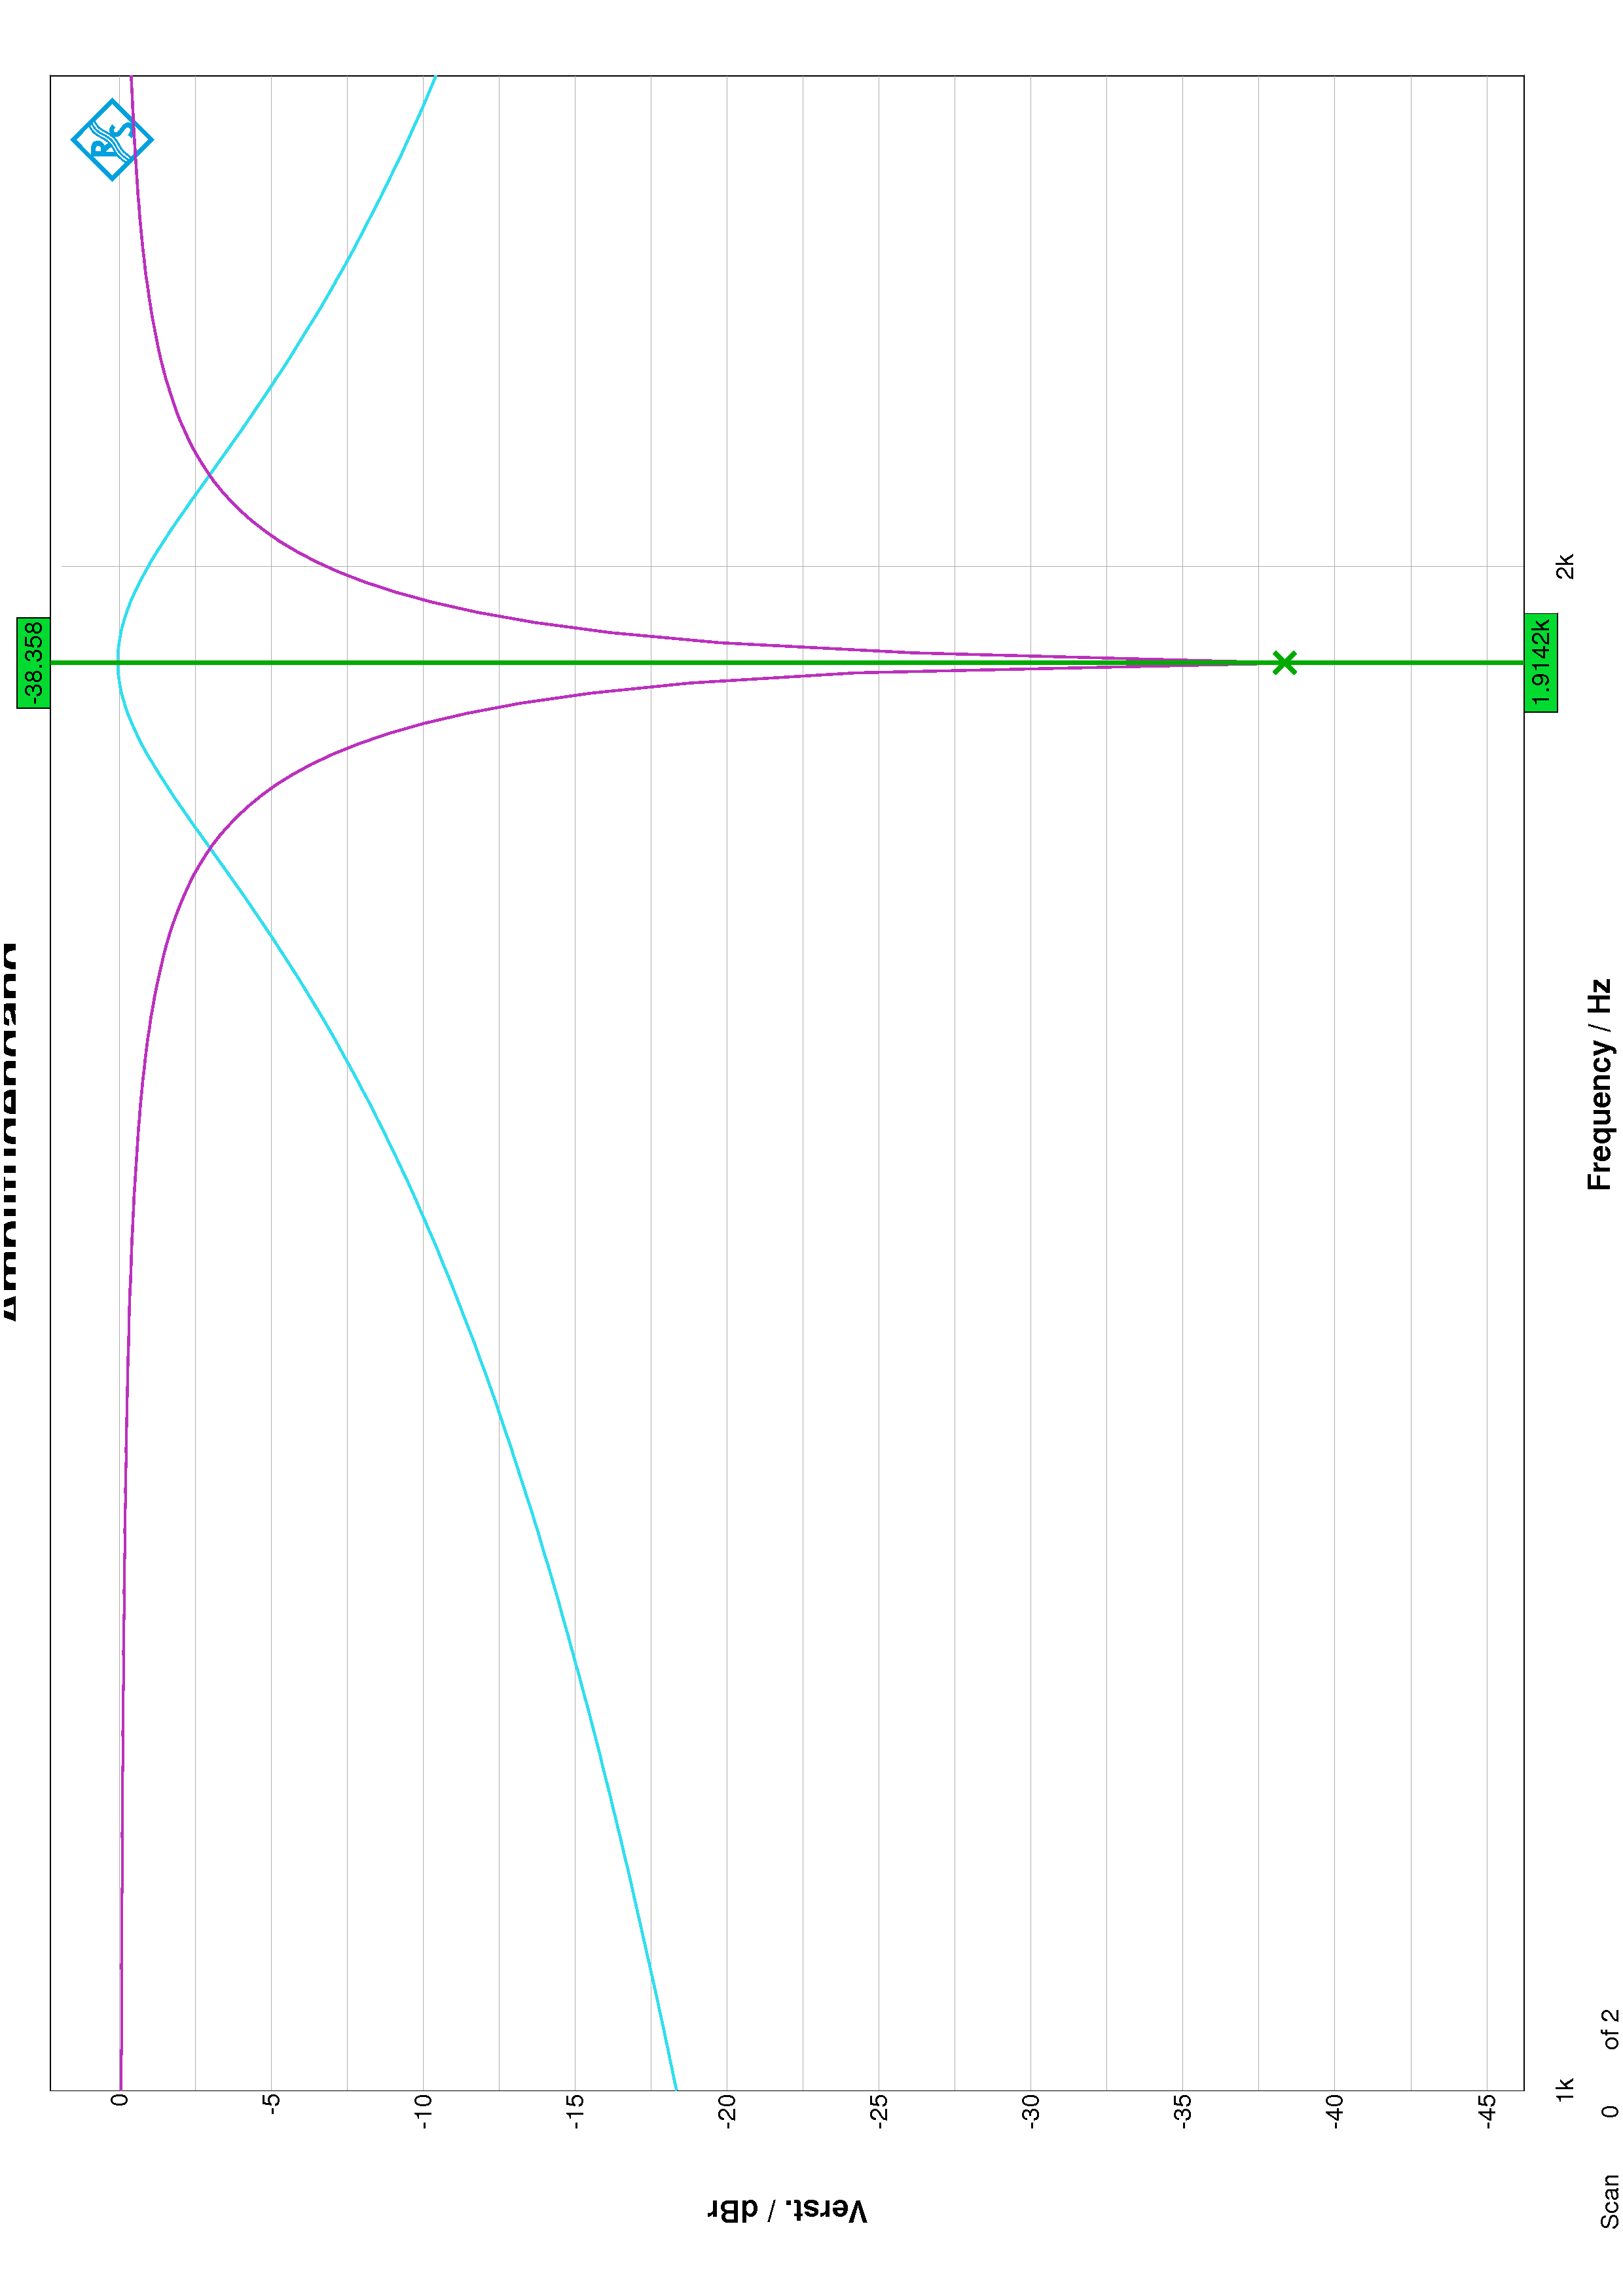
\includegraphics[width = \textwidth/3, angle =-90]{img/3.4 Amplitudengang Bandsperre.png}}\\
\subfloat[Bandbreite Bandpass]{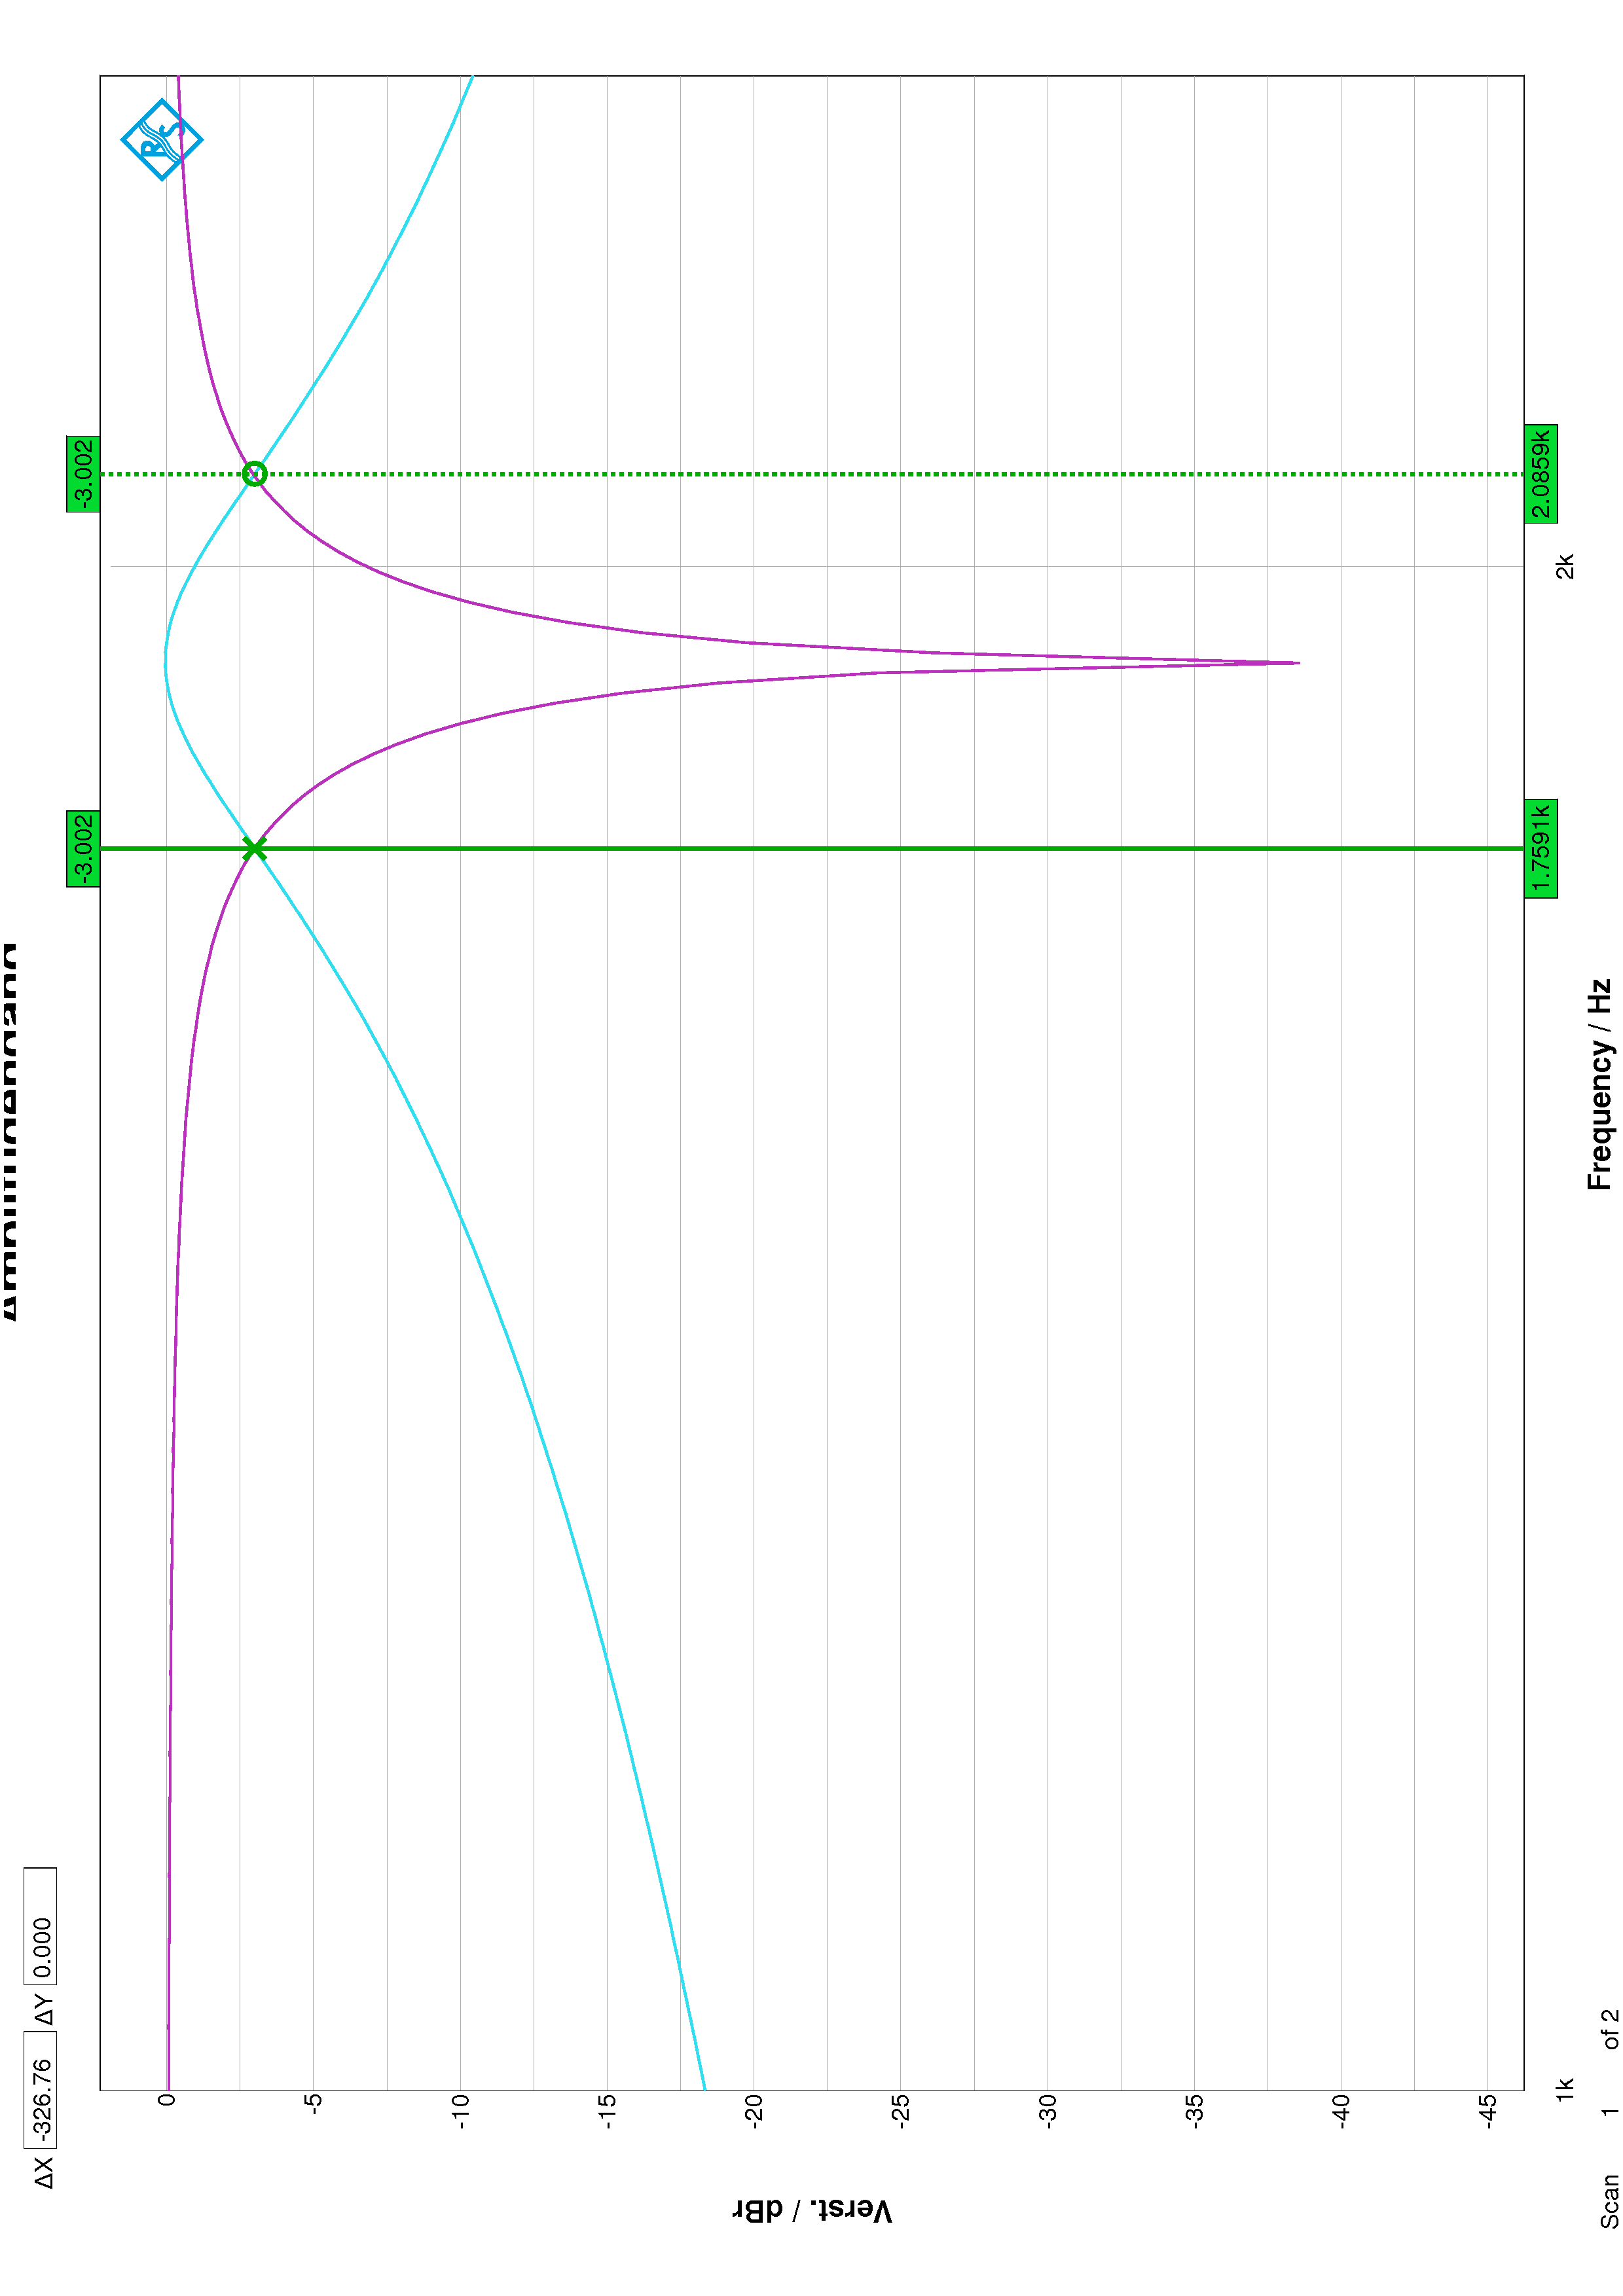
\includegraphics[width = \textwidth/3, angle =-90]{img/3.4 Bandbreite Bandpass.png}} 
\subfloat[Bandbreite Bandsperre]{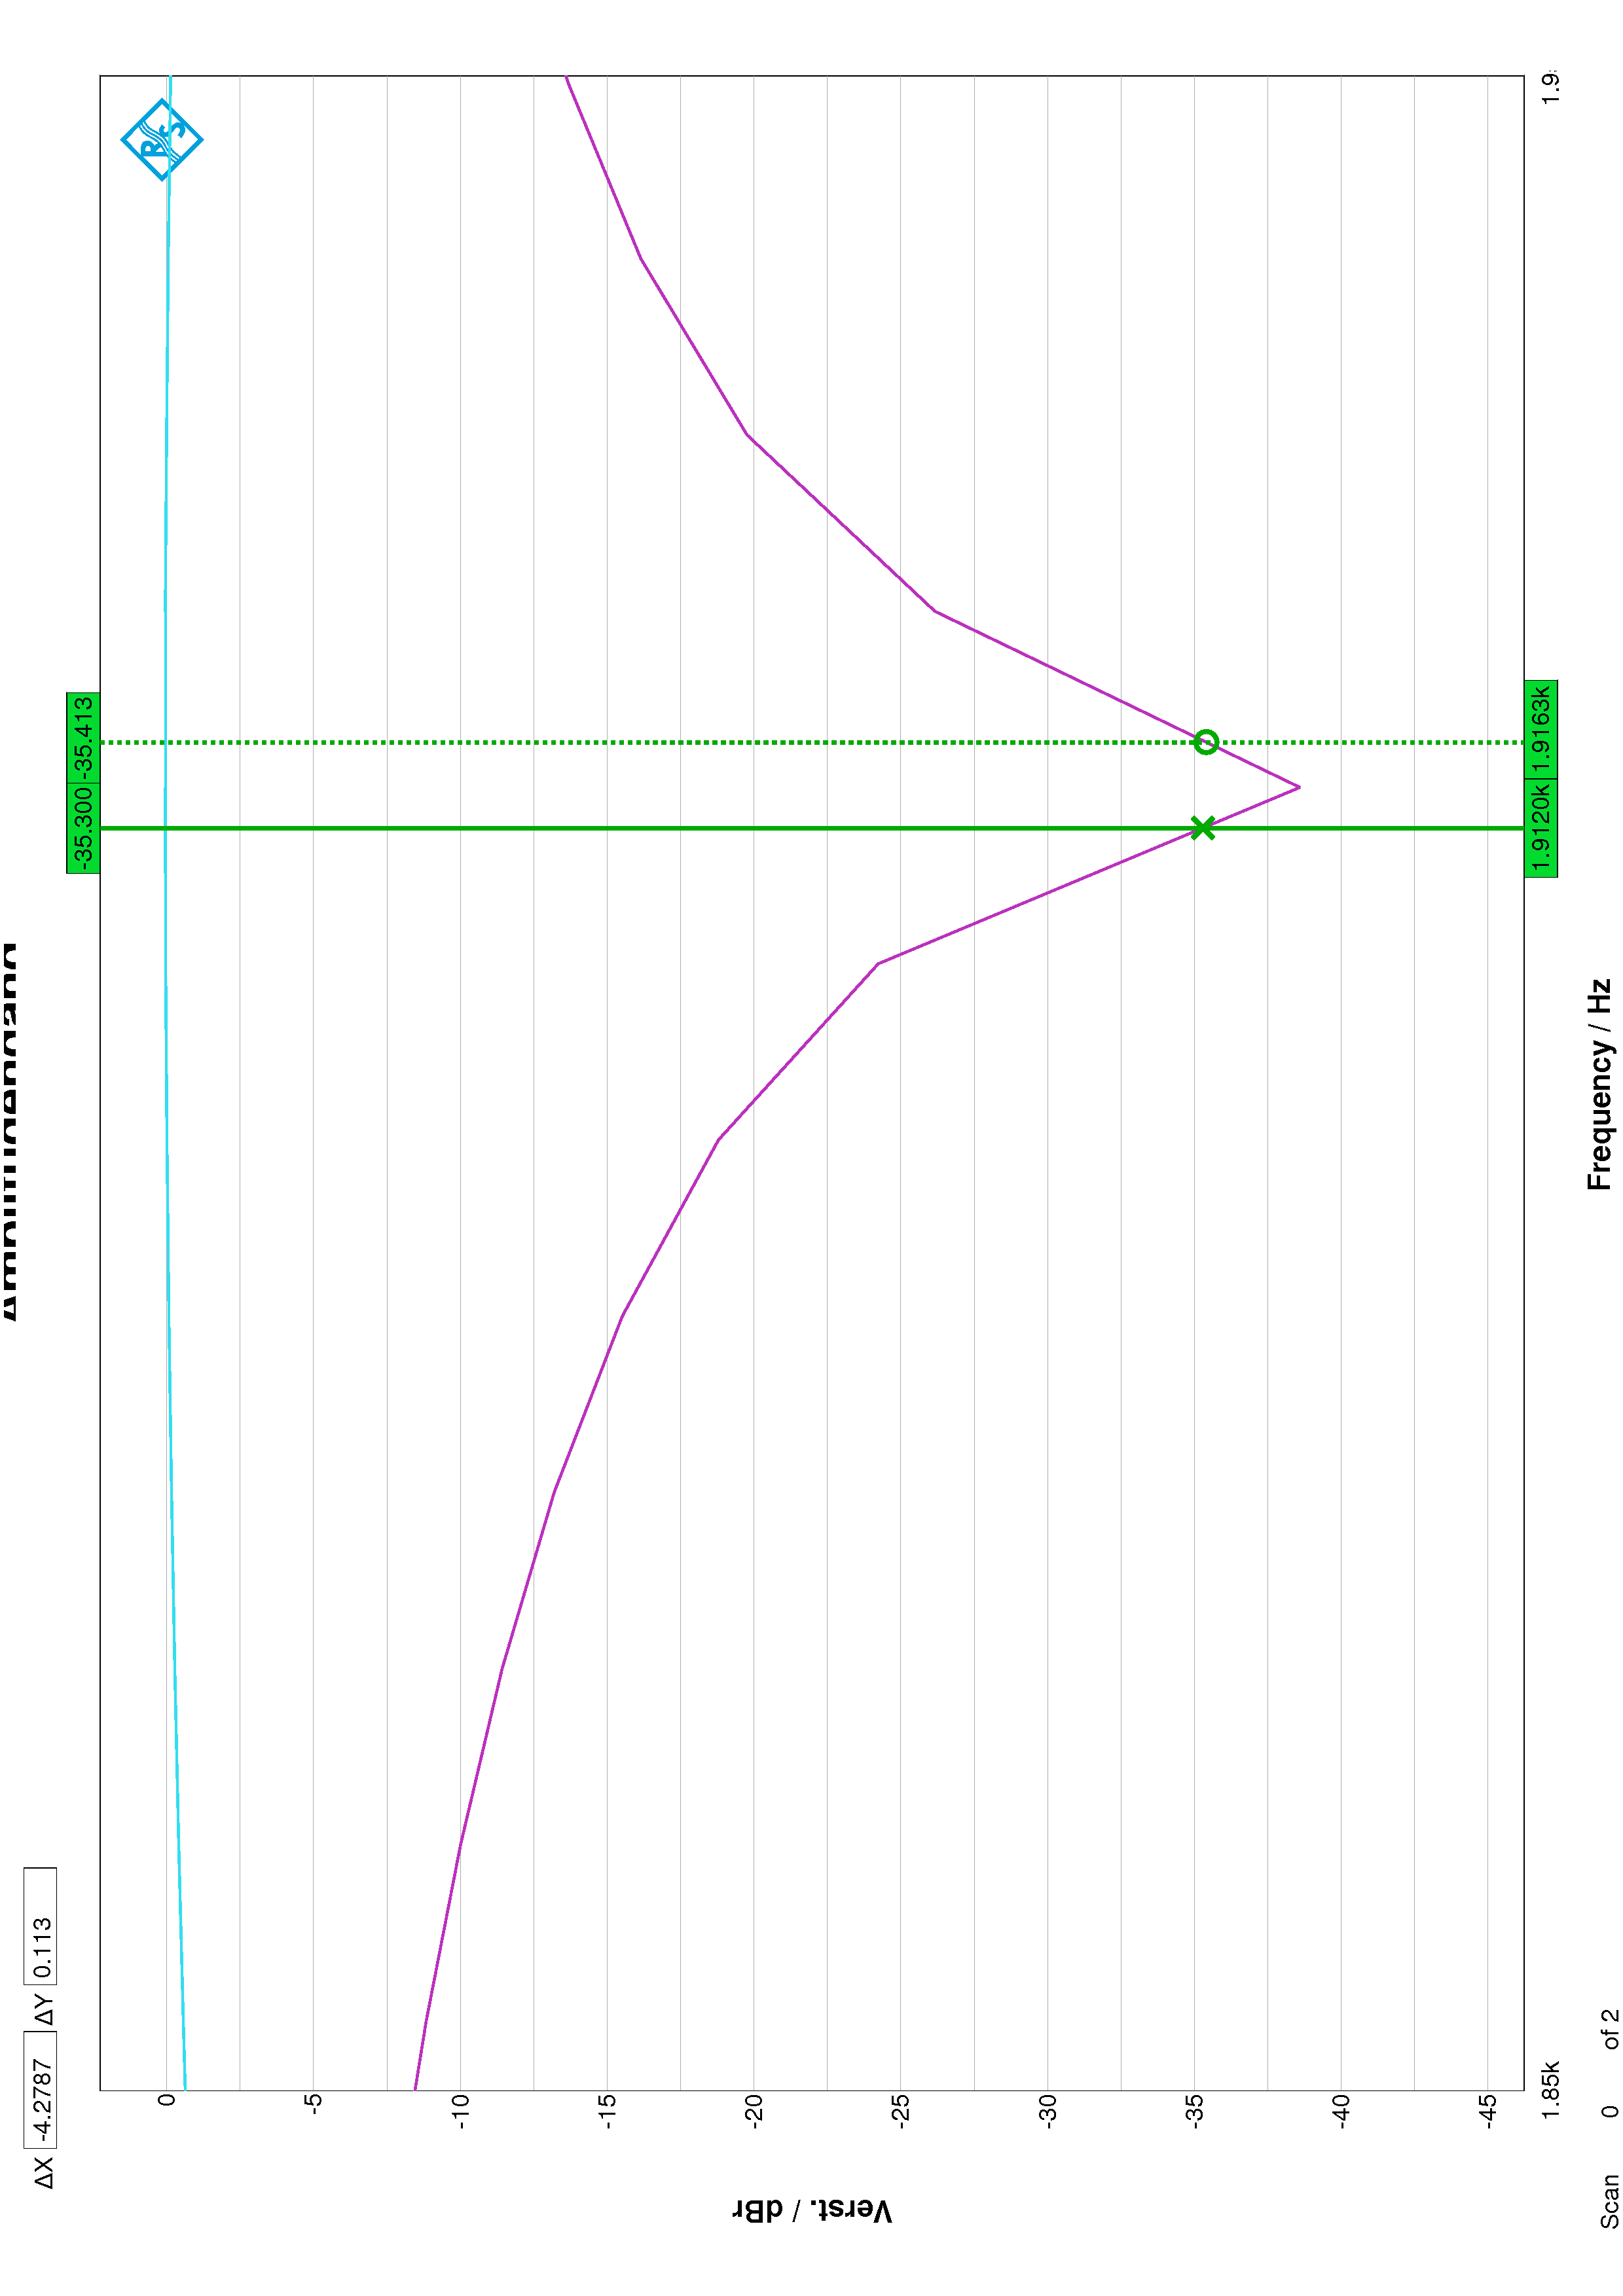
\includegraphics[width = \textwidth/3, angle =-90]{img/3.4 Bandbreite Bandsperre.png}} 
\caption{Bandbreiten}
\label{fig:A3_mult}
\end{center}
\end{figure}





























\subsection{Auswertung}
%%%%%%%%%%%%%%%%%%%%%%%%%%%%%%%%%%%%%%%%%%%%%%%%Comments
%Amplitudengänge von Butterworth-, Tschebyscheff- und Bessel-Tiefpass und Markierung der Grenzfrequenzen Phasengänge von Butterworth-, Tschebyscheff- und Bessel-Tiefpass und Markierung der Frequenzen für eine Phasenverschiebung von -60° und -120° Amplitudengänge von Butterworth-, Tschebyscheff- und Bessel-Hochpass und Markierung der Grenzfrequenzen Amplitudengänge von Bandpass und Bandsperre und Markierung der Grenzfrequenzen Auswertung: Alle Messwerte der Grenzfrequenzen sind in einer Tabelle mit den Vorgabewerten einzutragen und zu vergleichen; Aus den Frequenzen bei 60° und 120° Phasenverschiebung sind die Koeffizienten a1, b1 der 3 Tiefpässe zu berechnen und mit den Vorgabewerten zu vergleichen